% Sequence 2 : Symetrie centrale (5e)
\setseqtitle{Sym\'etrie centrale}
\chapter{Sym\'etrie centrale}

\begin{objectifsbox}
\textbf{Objectifs d'apprentissage.} À l'issue de la séquence, l'élève sera capable de :
\begin{itemize}
  \item Reconnaître et construire l'image d'une figure par symétrie centrale (centre donné)
  \item Utiliser les propriétés de conservation de la symétrie centrale
  \item Distinguer symétrie axiale et symétrie centrale
  \item Résoudre des problèmes géométriques en mobilisant la symétrie centrale
\end{itemize}
\end{objectifsbox}

\section{Rappel : symétrie axiale}

\begin{proprietebox}[Symétrie axiale]
La sym\'etrie axiale par rapport à une droite $d$ transforme tout point $M$ en un point $M'$ tel que $d$ est la médiatrice du segment $[MM']$. Elle conserve les longueurs, les angles et les aires.
\end{proprietebox}

\begin{examplebox}[Illustration]
\begin{center}
\begin{tikzpicture}[scale=0.9]
  % Axe de symetrie d (vertical)
  \draw[blue!60, very thick, dashed] (0,-2) -- (0,2) node[above]{$d$};
  % Points A et A' symetriques par rapport a d
  \coordinate (A) at (-2,1.2);
  \coordinate (Aprime) at (2,1.2);
  \draw[fill=black] (A) circle (1.5pt) node[above left]{$A$};
  \draw[fill=black] (Aprime) circle (1.5pt) node[above right]{$A'$};
  % Perpendiculaires
  \draw[gray,code1] (A) -- (0,1.2);
  \draw[gray,code1] (Aprime) -- (0,1.2);
\end{tikzpicture}
\end{center}
\end{examplebox}

\section{Découverte : symétrie centrale}

% Activité: deux symétries axiales successives
\begin{activitybox}[Deux symétries axiales pour une centrale]
\textbf{Consigne.}
\begin{enumerate}
  \item On considère deux droites \textbf{perpendiculaires} $d_1$ et $d_2$ qui se coupent en $I$.
  \item Construire une petite figure $F_0$ (par exemple un triangle ou la lettre \og L \fg{}).
  \item Construire $F_1$, image de $F_0$ par la symétrie axiale d'axe $d_1$.
  \item Construire $F_2$, image de $F_1$ par la symétrie axiale d'axe $d_2$.
  \item Comment passer directement de $F_0$ à $F_2$ sans pliage ni étape intermédiaire ?
\end{enumerate}

\begin{center}
	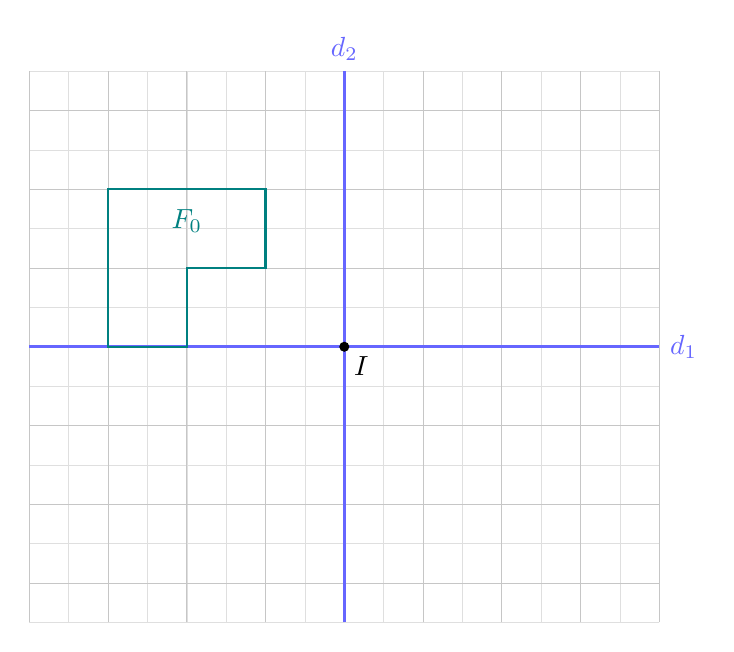
\begin{tikzpicture}[scale=1]
		% Grille (mineure 0.5, majeure 1)
		\draw[help lines, color=gray!25, step=0.5] (-4,-3.5) grid (4,3.5);
		\draw[help lines, color=gray!45, line width=0.25pt, step=1] (-4,-3.5) grid (4,3.5);
		
		% Axes perpendiculaires
		\coordinate (I) at (0,0);
		\draw[very thick, blue!60] (-4,0) -- (4,0) node[right]{$d_1$};
		\draw[very thick, blue!60] (0,-3.5) -- (0,3.5) node[above]{$d_2$};
		\draw[fill=black] (I) circle (1.6pt) node[below right]{$I$};
		
		% Figure F0 : lettre L, sommets sur la grille (entiers)
		\coordinate (P1) at (-3,2);
		\coordinate (P2) at (-1,2);
		\coordinate (P3) at (-1,1);
		\coordinate (P4) at (-2,1);
		\coordinate (P5) at (-2,0);
		\coordinate (P6) at (-3,0);
		\draw[thick, teal] (P1)--(P2)--(P3)--(P4)--(P5)--(P6)--cycle;
		\node[teal] at (-2,1.6) {$F_0$};
	\end{tikzpicture}
\end{center}

\trous{14cm}\\
\trous{14cm}\\
\trous{14cm}
\end{activitybox}


\begin{definitionbox}[Symétrie centrale]
	La \textbf{symétrie centrale} de centre $O$ est la transformation qui laisse $O$ invariant et qui transforme tout point $M$ en un point $M'$ tel que \textbf{$O$ est le milieu de $[MM']$}.
\end{definitionbox}

% L'ILLUSTRATION RESTE PARFAITE
\begin{examplebox}[Illustration]
	\begin{center}
		\begin{tikzpicture}[scale=1]
			\coordinate (O) at (0,0);
			\coordinate (M) at (2,1);
			\coordinate (M') at (-2,-1);
			\draw[fill=black] (O) circle (1.5pt) node[below right]{$O$};
			\draw[fill=black] (M) circle (1.5pt) node[above]{$M$};
			\draw[fill=black] (M') circle (1.5pt) node[below]{$M'$};
			\draw[gray] (M) -- (M');
			% Suggestion d'amélioration pour le placement du mot "milieu"
			\node[anchor=south west, xshift=1pt, yshift=1pt, inner sep=1pt, fill=white] at (O) {\small milieu};
		\end{tikzpicture}
	\end{center}
\end{examplebox}

\section{Figures symétriques par rapport à un point}
\begin{definitionbox}
Deux figures sont symétriques par rapport à un point $O$ lorsqu'elles \\
se superposent en \trous{10cm}\\
autour de ce point.
On dit que $O$ est le centre de la symétrie.
\end{definitionbox}

\begin{examplebox}
	\begin{center}
		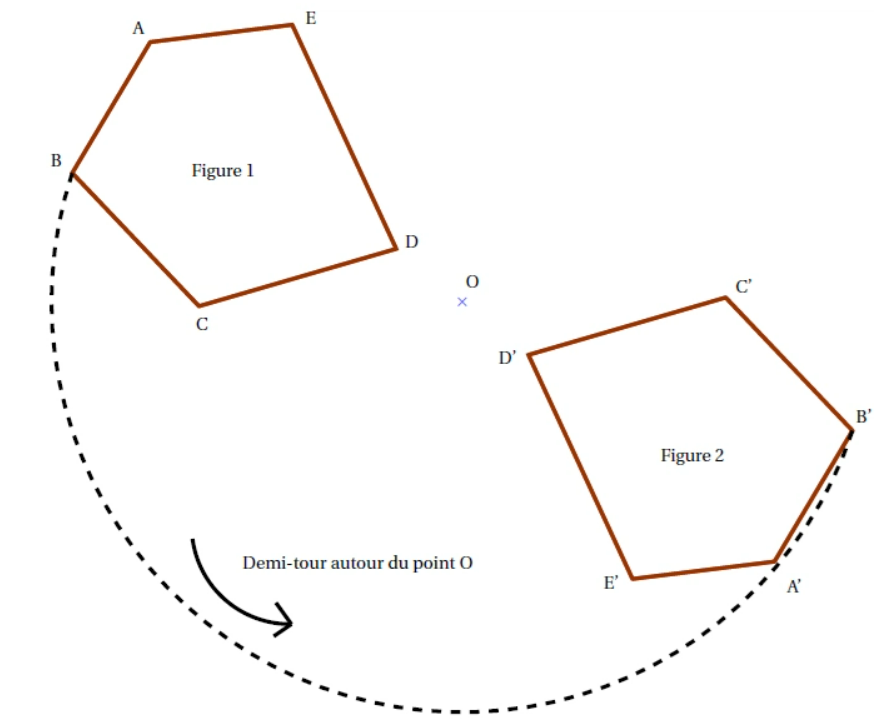
\includegraphics[width=0.6\linewidth]{../../assets/images/5e/seq_02/figures_symetriques}
	\end{center}
	
\end{examplebox}	

\section{Symétrique d'un point par rapport à un point}

\begin{definitionbox}
	Le symétrique d’un point $M$ par rapport à un point $O$ est le point $M'$ tel que le point $O$ est le milieu du segment $[MM']$.
\end{definitionbox}

\begin{examplebox}
	Placer le symétrique $A'$ du point $A$ par rapport au point $O$ en utilisant le quadrillage.
	\begin{center}
		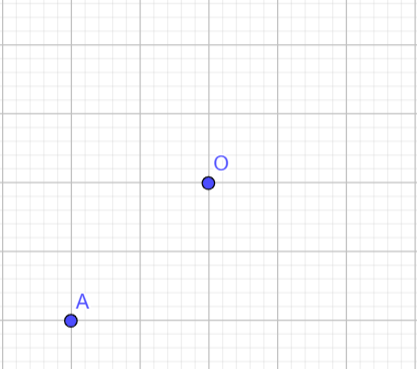
\includegraphics[width=0.7\linewidth]{../../assets/images/5e/seq_02/exemple_image_point_construction}
	\end{center}
	

\end{examplebox}	

\section{Constructions}

\subsection{Image d'un point}
\begin{methodebox}[Point à point]
Pour construire l'image $A'$ d'un point $A$ par la symétrie centrale de centre $O$ :
\begin{enumerate}
  \item Tracer la demi-droite $[AO)$.
  \item Reporter $OA$ de l'autre côté de $O$ pour obtenir le point $A'$ avec $OA'=OA$ (à la règle et au compas).
  \item Vérifier que $O$ est le milieu de $[AA']$.
\end{enumerate}


\begin{center}
	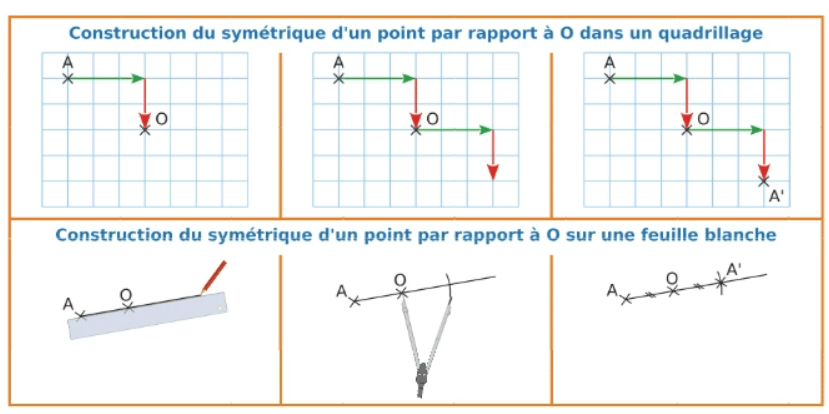
\includegraphics[width=1\linewidth]{../../assets/images/5e/seq_02/methode_construction_point_par_symetrie_centrale}
\end{center}

\end{methodebox}



\subsection{Image d'une figure}
\begin{methodebox}[Segment, droite, triangle]
\begin{itemize}
  \item \textbf{Segment $[AB]$} \;$\to$\; \textit{$[A'B']$ parall\`ele et de m\^eme longueur}.
  \item \textbf{Droite $(d)$} \;$\to$\; \textit{droite $d'$ parallèle à $(d)$} (si $(d)$ passe par $O$, elle est invariante).
  \item \textbf{Triangle $ABC$} \;$\to$\; \textit{triangle $A'B'C'$ superposable par demi-tour (aires et angles conserv\'es)}.
\end{itemize}
\end{methodebox}

\begin{examplebox}[Construction par symétrie centrale]
	Construire l’image du triangle $ABC$ par la symétrie centrale de centre $O$. Laisser visibles les traits de construction et nommer $A'$, $B'$, $C'$.
	
	\begin{center}
		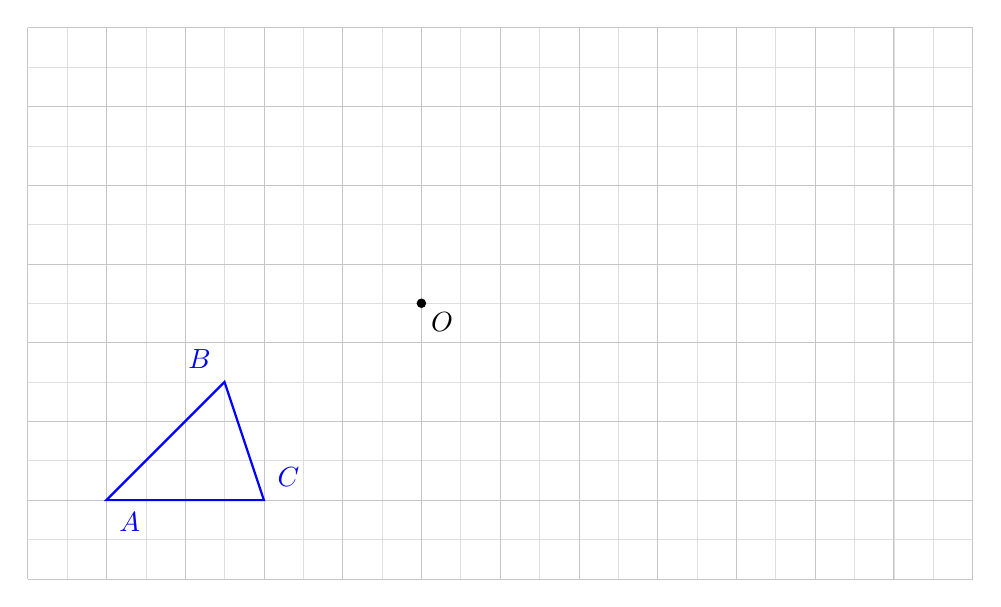
\begin{tikzpicture}[x=1cm,y=1cm]
			% Zone de dessin
			\useasboundingbox (0,0) rectangle (12,7);
			
			% Quadrillage (mineur 0.5, majeur 1)
			\draw[help lines, color=gray!25, step=0.5] (0,0) grid (12,7);
			\draw[help lines, color=gray!45, line width=0.25pt, step=1] (0,0) grid (12,7);
			
			% Centre O (au centre)
			\coordinate (O) at (5,3.5);
			\draw[fill=black] (O) circle (1.5pt);
			\node[below right] at (O) {$O$};
			
			% Triangle ABC en bas à gauche (sommets sur la grille)
			\coordinate (A) at (1,1);
			\coordinate (B) at (2.5,2.5);
			\coordinate (C) at (3,1);
			\draw[thick, blue] (A)--(B)--(C)--cycle;
			
			% Étiquettes bien placées
			\node[below right, xshift=0.4mm, yshift=-0.4mm, blue] at (A) {$A$};
			\node[above left, xshift=-0.5mm, yshift=0.5mm, blue] at (B) {$B$};
			\node[above right, xshift=0.5mm, yshift=0.5mm, blue] at (C) {$C$};
		\end{tikzpicture}
	\end{center}
\end{examplebox}

\section{Propriétés}

\begin{proprietebox}[Conservations]
La sym\'etrie centrale (centre $O$) :
\begin{itemize}
  \item conserve les longueurs, les angles et les aires ;
  \item envoie une droite ne passant pas par $O$ sur une droite \textbf{parall\`ele} ;
  \item laisse inchang\'ee toute droite passant par $O$ ;
  \item transforme un cercle en un cercle de m\^eme rayon ;
  \item est \textbf{\'equivalente au demi-tour} (rotation d'angle $180^{\circ}$) de centre $O$.
\end{itemize}
\end{proprietebox}

\begin{remarkbox}
Une figure qui admet un centre de sym\'etrie est dite \textbf{centrosym\'etrique} (ex. : parall\'elogramme, rectangle, losange, cercle).
\end{remarkbox}

\section{Centre de symétrie d'une figure}

\begin{definitionbox}[Centre de symétrie]
Une figure $\mathcal F$ \textbf{admet un centre de symétrie} s'il existe un point $O$ tel que la symétrie centrale de centre $O$ laisse $\mathcal F$ \textbf{inchangée} (chaque point de $\mathcal F$ a son image encore dans $\mathcal F$). On dit alors que $O$ est \textbf{centre de symétrie} de $\mathcal F$.
\end{definitionbox}

\begin{examplebox}[Exemples et contre-exemples]
\begin{itemize}
  \item Segment $[AB]$ : centre $I$, \textbf{milieu} de $[AB]$.
  \item Cercle ou disque : \textbf{son centre}.
  \item Parallélogramme, rectangle, losange : \textbf{intersection des diagonales}.
  \item Triangle quelconque, lettre \og L\fg{} : \textbf{pas} de centre de symétrie.
\end{itemize}

\begin{center}
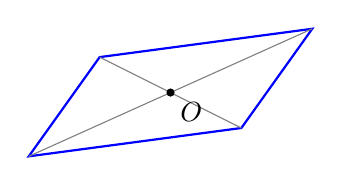
\begin{tikzpicture}[scale=0.9]
  % Parallélogramme avec centre
  \coordinate (A) at (0,0);
  \coordinate (B) at (3,0.4);
  \coordinate (C) at (4,1.8);
  \coordinate (D) at (1,1.4);
  \draw[thick,blue] (A)--(B)--(C)--(D)--cycle;
  \draw[gray] (A)--(C) (B)--(D);
  \path (A)--(C) coordinate[pos=0.5] (O);
  \draw[fill=black] (O) circle (1.4pt) node[below right]{$O$};
\end{tikzpicture}
\end{center}
\end{examplebox}

\begin{methodebox}[Comment le trouver ?]
\begin{itemize}
  \item \textbf{Segment} : prendre le \textbf{milieu}.
  \item \textbf{Parallélogramme/rectangle/losange} : tracer les \textbf{deux diagonales} et prendre leur \textbf{intersection}.
  \item \textbf{Cercle/disque} : le \textbf{centre} du cercle.
  \item \textbf{Polygone régulier à nombre pair de côtés} : centre du polygone. À nombre impair : \textbf{pas} de centre de symétrie.
\end{itemize}
\end{methodebox}

%\begin{proprietebox}[Unicité et cas particuliers]
%Pour une figure \textbf{bornée} (segment, polygone, disque, etc.), s'il existe, le centre de symétrie est en général \textbf{unique}. Une \textbf{droite} admet au contraire une infinité de centres : \textbf{tous ses points}.
%\end{proprietebox}

\clearpage
\section{Comparaison : axiale vs centrale}

\begin{methodebox}[Comment les distinguer ?]
\begin{itemize}
  \item \textbf{Axiale} : on cherche une \textit{droite} qui partage la figure en deux parties superposables.
  \item \textbf{Centrale} : on cherche un \textit{point $O$} tel que toute droite passant par $O$ coupe la figure en deux points sym\'etriques (milieu en $O$).
\end{itemize}
\end{methodebox}

\section{Exercices d'application}

\begin{exercisebox}
\textbf{Exercice 1 (construction)}. On donne un point $O$ et des points $A$, $B$, $C$.
\begin{enumerate}
  \item Construire $A'$, $B'$, $C'$ images de $A$, $B$, $C$ par la sym\'etrie centrale de centre $O$.
  \item Que peut-on dire des segments $[AB]$ et $[A'B']$ ? des angles $\widehat{ABC}$ et $\widehat{A'B'C'}$ ?
\end{enumerate}
\end{exercisebox}

\begin{exercisebox}
\textbf{Exercice 2 (triangle)}. Construire l'image du triangle $ABC$ par la sym\'etrie centrale de centre $O$. Tracer ensuite les droites $(AA')$, $(BB')$, $(CC')$ : que remarquez-vous ?
\end{exercisebox}

\begin{exercisebox}
\textbf{Exercice 3 (droites et cercles)}. Soit une droite $(d)$ qui ne passe pas par $O$ et un cercle $\mathcal C$ de centre $A$ passant par $B$.
\begin{enumerate}
  \item Construire l'image $(d')$ de $(d)$.
  \item Construire l'image $\mathcal C'$ de $\mathcal C$ et pr\'eciser son centre et son rayon.
\end{enumerate}
\end{exercisebox}

\begin{exercisebox}
\textbf{Exercice 4 (vrai/faux)}. Dire si les affirmations sont vraies ou fausses et justifier.
\begin{enumerate}
  \item Par sym\'etrie centrale, un rectangle devient un parall\'elogramme.
  \item L'image d'une droite par une sym\'etrie centrale est toujours la même droite.
  \item Si $ABCD$ est un parall\'elogramme, alors $O$, intersection des diagonales, est un centre de sym\'etrie.
\end{enumerate}
\end{exercisebox}

\begin{quizbox}
\textbf{Auto-\'evaluation rapide}
\begin{enumerate}[label=\arabic*)]
  \item Donner la d\'efinition de l'image d'un point par sym\'etrie centrale.
  \item Citer deux propri\'et\'es conserv\'ees par la sym\'etrie centrale.
  \item Expliquer comment distinguer visuellement une symétrie axiale d'une symétrie centrale.
\end{enumerate}
\end{quizbox}

\clearpage
\section*{Corrigés des exercices d'application}

\begin{solutionbox}
	\textbf{Exercice 1 — Correction}
	\begin{enumerate}
		\item Pour construire l'image de chaque point ($A$, $B$ ou $C$) :
		\begin{itemize}
			\item Tracer la droite passant par $O$ et le point (par exemple $A$).
			\item Placer le point image $A'$ de l'autre côté de $O$, à la même distance : $OA' = OA$.
			\item Ainsi, $O$ est le milieu du segment $[AA']$.
			\item Faire de même pour $B$ et $C$.
		\end{itemize}

		\begin{center}
		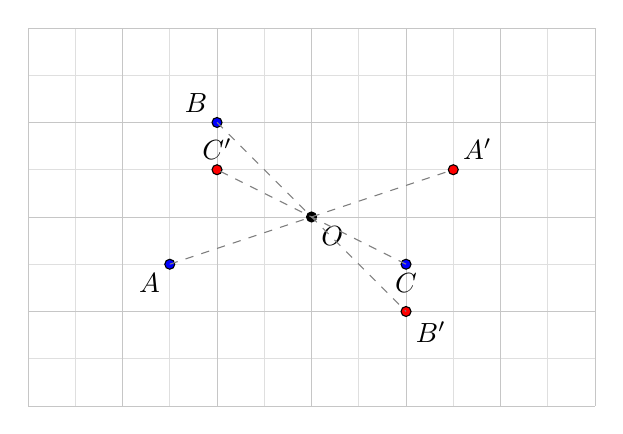
\begin{tikzpicture}[scale=1.2]
			% Grille
			\draw[help lines, color=gray!25, step=0.5] (-1,-1) grid (5,3);
			\draw[help lines, color=gray!45, line width=0.25pt, step=1] (-1,-1) grid (5,3);

			% Centre O
			\coordinate (O) at (2,1);
			\draw[fill=black] (O) circle (1.5pt) node[below right]{$O$};

			% Points A, B, C
			\coordinate (A) at (0.5,0.5);
			\coordinate (B) at (1,2);
			\coordinate (C) at (3,0.5);
			\draw[fill=blue] (A) circle (1.5pt) node[below left]{$A$};
			\draw[fill=blue] (B) circle (1.5pt) node[above left]{$B$};
			\draw[fill=blue] (C) circle (1.5pt) node[below]{$C$};

			% Images A', B', C'
			\coordinate (A') at (3.5,1.5);
			\coordinate (B') at (3,0);
			\coordinate (C') at (1,1.5);
			\draw[fill=red] (A') circle (1.5pt) node[above right]{$A'$};
			\draw[fill=red] (B') circle (1.5pt) node[below right]{$B'$};
			\draw[fill=red] (C') circle (1.5pt) node[above]{$C'$};

			% Droites de construction
			\draw[gray, dashed] (A) -- (A');
			\draw[gray, dashed] (B) -- (B');
			\draw[gray, dashed] (C) -- (C');
		\end{tikzpicture}
		\end{center}

		\item Les segments $[AB]$ et $[A'B']$ ont la même longueur et sont parallèles. De même, les angles $\widehat{ABC}$ et $\widehat{A'B'C'}$ ont la même mesure (la symétrie centrale conserve les longueurs et les angles).
	\end{enumerate}
\end{solutionbox}

\begin{solutionbox}
	\textbf{Exercice 2 — Correction}

	On construit l'image du triangle $ABC$ en trouvant les points $A'$, $B'$, $C'$ images de $A$, $B$, $C$ par la symétrie centrale de centre $O$.

	\begin{center}
	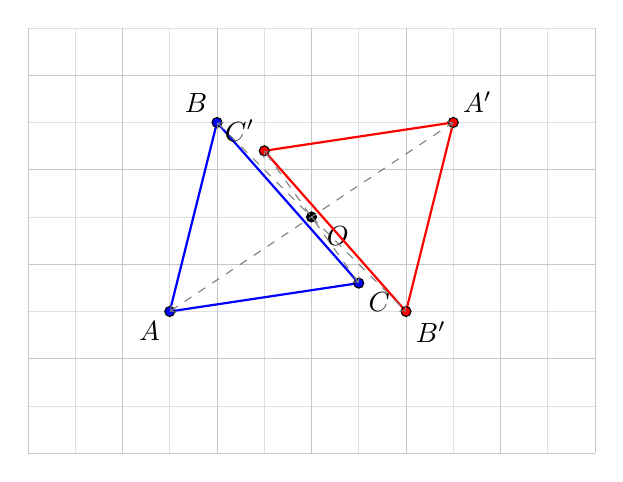
\begin{tikzpicture}[scale=1.2]
		% Grille
		\draw[help lines, color=gray!25, step=0.5] (-1,-1) grid (5,3.5);
		\draw[help lines, color=gray!45, line width=0.25pt, step=1] (-1,-1) grid (5,3.5);

		% Centre O
		\coordinate (O) at (2,1.5);
		\draw[fill=black] (O) circle (1.5pt) node[below right, xshift=2pt]{$O$};

		% Triangle ABC
		\coordinate (A) at (0.5,0.5);
		\coordinate (B) at (1,2.5);
		\coordinate (C) at (2.5,0.8);
		\draw[thick, blue] (A) -- (B) -- (C) -- cycle;
		\draw[fill=blue] (A) circle (1.5pt) node[below left]{$A$};
		\draw[fill=blue] (B) circle (1.5pt) node[above left]{$B$};
		\draw[fill=blue] (C) circle (1.5pt) node[below right]{$C$};

		% Triangle A'B'C'
		\coordinate (A') at (3.5,2.5);
		\coordinate (B') at (3,0.5);
		\coordinate (C') at (1.5,2.2);
		\draw[thick, red] (A') -- (B') -- (C') -- cycle;
		\draw[fill=red] (A') circle (1.5pt) node[above right]{$A'$};
		\draw[fill=red] (B') circle (1.5pt) node[below right]{$B'$};
		\draw[fill=red] (C') circle (1.5pt) node[above left]{$C'$};

		% Droites passant par O
		\draw[gray, dashed, <->] (A) -- (A');
		\draw[gray, dashed, <->] (B) -- (B');
		\draw[gray, dashed, <->] (C) -- (C');
	\end{tikzpicture}
	\end{center}

	\textbf{Observation :} Les trois droites $(AA')$, $(BB')$ et $(CC')$ passent toutes par le point $O$. En effet, $O$ est le milieu de chaque segment $[AA']$, $[BB']$ et $[CC']$, donc toutes ces droites se coupent en $O$.
\end{solutionbox}

\begin{solutionbox}
	\textbf{Exercice 3 — Correction}
	\begin{enumerate}
		\item Pour construire l'image $(d')$ de la droite $(d)$ :
		\begin{itemize}
			\item Choisir deux points sur $(d)$, par exemple $P$ et $Q$.
			\item Construire leurs images $P'$ et $Q'$ par la symétrie de centre $O$.
			\item La droite $(d')$ passe par $P'$ et $Q'$.
			\item Puisque $(d)$ ne passe pas par $O$, la droite $(d')$ est parallèle à $(d)$.
		\end{itemize}

		\begin{center}
		\begin{tikzpicture}[scale=1.1]
			% Grille
			\draw[help lines, color=gray!25, step=0.5] (-0.5,-0.5) grid (6,3.5);
			\draw[help lines, color=gray!45, line width=0.25pt, step=1] (-0.5,-0.5) grid (6,3.5);

			% Centre O
			\coordinate (O) at (2.5,1.5);
			\draw[fill=black] (O) circle (1.5pt) node[below right]{$O$};

			% Droite (d) et points P, Q
			\coordinate (P) at (0.5,0.8);
			\coordinate (Q) at (2,0.3);
			\draw[thick, blue] (0,1) -- (3,0) node[right]{$(d)$};
			\draw[fill=blue] (P) circle (1.5pt) node[above left]{$P$};
			\draw[fill=blue] (Q) circle (1.5pt) node[above right]{$Q$};

			% Images P' et Q' par symétrie de centre O
			\coordinate (P') at (4.5,2.2);
			\coordinate (Q') at (3,2.7);
			\draw[fill=red] (P') circle (1.5pt) node[below right]{$P'$};
			\draw[fill=red] (Q') circle (1.5pt) node[below left]{$Q'$};

			% Droite (d') passant par P' et Q'
			\draw[thick, red] ($(P')!-0.3!(Q')$) -- ($(Q')!-0.3!(P')$) node[right]{$(d')$};

			% Droites de construction
			\draw[gray, dashed] (P) -- (P');
			\draw[gray, dashed] (Q) -- (Q');
		\end{tikzpicture}
		\end{center}

		\item Pour construire l'image $\mathcal C'$ du cercle $\mathcal C$ :
		\begin{itemize}
			\item Trouver l'image $A'$ du centre $A$ par la symétrie de centre $O$.
			\item Le cercle $\mathcal C'$ a pour centre $A'$.
			\item Son rayon est le même que celui de $\mathcal C$, c'est-à-dire $AB$ (ou $A'B' = AB$).
		\end{itemize}

		\begin{center}
		\begin{tikzpicture}[scale=1.1]
			% Grille
			\draw[help lines, color=gray!25, step=0.5] (-0.5,-0.5) grid (6,3.5);
			\draw[help lines, color=gray!45, line width=0.25pt, step=1] (-0.5,-0.5) grid (6,3.5);

			% Centre O
			\coordinate (O) at (3,1.5);
			\draw[fill=black] (O) circle (1.5pt) node[below right]{$O$};

			% Cercle C
			\coordinate (A) at (1.5,1);
			\draw[thick, blue] (A) circle (0.7cm);
			\draw[fill=blue] (A) circle (1.5pt) node[below left]{$A$};
			% B sur le cercle : angle 45 degrés, rayon 0.7cm
			\coordinate (B) at ($(A) + (45:0.7cm)$);
			\draw[fill=blue] (B) circle (1.5pt) node[above right]{$B$};
			\node[blue] at (1.5,0) {$\mathcal C$};

			% Cercle C' (image de C par symétrie de centre O)
			\coordinate (A') at (4.5,2);
			\draw[thick, red] (A') circle (0.7cm);
			\draw[fill=red] (A') circle (1.5pt) node[above right]{$A'$};
			% B' image de B par symétrie de centre O : B' = 2*O - B
			\coordinate (B') at ($(2*3,2*1.5) - (B)$);
			\draw[fill=red] (B') circle (1.5pt) node[below left]{$B'$};
			\node[red] at (4.5,3) {$\mathcal C'$};

			% Droites de construction
			\draw[gray, dashed] (A) -- (A');
			\draw[gray, dashed] (B) -- (B');
		\end{tikzpicture}
		\end{center}
	\end{enumerate}
\end{solutionbox}

\begin{solutionbox}
	\textbf{Exercice 4 — Correction}
	\begin{enumerate}
		\item \textbf{Vrai.} Un rectangle reste un rectangle par symétrie centrale (donc c'est aussi un parallélogramme).

		\item \textbf{Faux.} L'image d'une droite par symétrie centrale est la même droite seulement si la droite passe par le centre $O$. Sinon, l'image est une droite parallèle mais différente.

		\item \textbf{Vrai.} Dans un parallélogramme $ABCD$, le point $O$ (intersection des diagonales) est un centre de symétrie : il échange les sommets opposés ($A$ avec $C$, et $B$ avec $D$).

		\begin{center}
		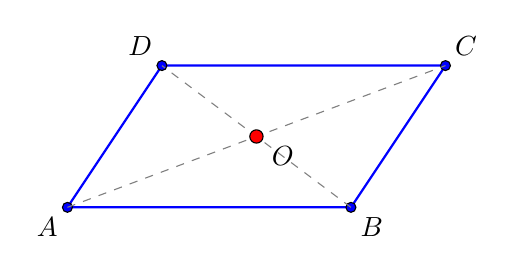
\begin{tikzpicture}[scale=1.2]
			% Parallélogramme ABCD
			\coordinate (A) at (0,0);
			\coordinate (B) at (3,0);
			\coordinate (C) at (4,1.5);
			\coordinate (D) at (1,1.5);
			\draw[thick, blue] (A) -- (B) -- (C) -- (D) -- cycle;
			\draw[fill=blue] (A) circle (1.5pt) node[below left]{$A$};
			\draw[fill=blue] (B) circle (1.5pt) node[below right]{$B$};
			\draw[fill=blue] (C) circle (1.5pt) node[above right]{$C$};
			\draw[fill=blue] (D) circle (1.5pt) node[above left]{$D$};

			% Diagonales
			\draw[gray, dashed] (A) -- (C);
			\draw[gray, dashed] (B) -- (D);

			% Centre O
			\coordinate (O) at (2,0.75);
			\draw[fill=red] (O) circle (2pt) node[below right, xshift=2pt]{$O$};
		\end{tikzpicture}
		\end{center}
	\end{enumerate}
\end{solutionbox}

\begin{solutionbox}
	\textbf{Auto-évaluation rapide — Corrigé}
	\begin{enumerate}[label=\arabic*)]
		\item L'image d'un point $M$ par la symétrie centrale de centre $O$ est le point $M'$ tel que $O$ soit le milieu du segment $[MM']$.
		\item Propriétés conservées : longueurs, mesures d'angles, alignement, parallélisme, aires.
		\item \textbf{Symétrie axiale :} on plie la figure le long d'une droite (l'axe). \textbf{Symétrie centrale :} on fait tourner la figure d'un demi-tour autour d'un point (le centre).
	\end{enumerate}
\end{solutionbox}

